%=====================================================================
% main.tex
%=====================================================================
% This file contains:
%	- Document Class
%	- Packages
%	- Format Information
%	- Custom Commands
%	- Chapters
%	- Bibliography
%	- Appendices
%	- Curriculum Vita

%=====================================================================
% Document Style
%=====================================================================
% The margincheck option flags lines which overflow their hbox with a black
%  box at the end of the line.  This usually (but not always) indicates a
%  margin violation on the right margin.  Left margin violations aren't
%  indicated and if the margin violation is large enough, there isn't room
%  for the black box to be visiable.  

% A 12 Point UW PhD Thesis.
 \listfiles
\documentclass[margincheck]{withesis}

%=====================================================================
% Packageges
%=====================================================================
\usepackage[usenames,dvipsnames,svgnames,table]{xcolor}
\usepackage{epsfig}
\usepackage{amssymb,amsmath}
\usepackage{verbatim}
\usepackage{tikz}
\usetikzlibrary{shapes}
\usetikzlibrary{arrows}
\usetikzlibrary{patterns}

\usepackage{times}
\renewcommand{\ttdefault}{cmtt}

\usepackage{subfig}

\usepackage{IEEEtrantools}
\usepackage{algpseudocode}
\usepackage{pdflscape}
\usepackage[absolute]{textpos}

\usepackage{fancyhdr}
\setlength{\TPHorizModule}{1in}
\setlength{\TPVertModule}{1in}
\fancypagestyle{lscape}{% 
\fancyhf{} % clear all header and footer fields 
\fancyfoot[LO]{\begin{textblock}{1}(1,   1){\rotatebox{90}{\thepage}}\end{textblock}}
\fancyfoot[LE]{\begin{textblock}{1}(1,10.5){\rotatebox{90}{\thepage}}\end{textblock}}
}
\renewcommand{\headrulewidth}{0pt} 
\renewcommand{\footrulewidth}{0pt}

\usepackage[numbers, sort&compress]{natbib}
\renewcommand{\bibname}{List of References}
\let\oldbibsection\bibsection
\renewcommand{\bibsection}{\oldbibsection\addcontentsline{toc}{chapter}{List of References}\singlespace\raggedright}

\usepackage{booktabs}
\usepackage{multirow}
\usepackage{lipsum}

\usepackage[bookmarks,
	bookmarksdepth=2,
	pdfauthor={Lewis John Lloyd}, %
	colorlinks, %
	citecolor=black, %
	filecolor=black, %
	linkcolor=black, %
	urlcolor=black]{hyperref}

\pagestyle{thesis}
%\draftscreen
\setcounter{errorcontextlines}{999}

% Include custom math commands
%============================================================================
% commands.tex
%============================================================================
% This file contains:
% 	- Defined Variables
%	- Redefined math shorthand
%	- Defined math shorthand


%============================================================================
% Redefined Math Commands
%============================================================================
% 	- \Vec{1} or \vec{1}
%		Long Name: Vector
%		Arguements[1]: bold and overbar arg1	
\DeclareRobustCommand{\Vec}[1]{%
    \ifmmode
        \mathbf{#1}\,%
    \else
        $\displaystyle \mathbf{#1}\,$%
    \fi
}
\DeclareRobustCommand{\vec}[1]{\Vec{#1}}

\DeclareRobustCommand{\lbm}{%
    \ifmmode
        \text{lb}_{\text{m}}
    \else
        $\displaystyle \text{lb}_{\text{m}}$%
    \fi
}
\DeclareRobustCommand{\lbf}{%
    \ifmmode
        \text{lb}_{\text{f}}
    \else
        $\displaystyle \text{lb}_{\text{f}}$
    \fi
}
\DeclareRobustCommand{\dt}{%
	\ifmmode
		\Delta t
	\else
		$\Delta t$
	\fi
}
\DeclareRobustCommand{\dtmax}{%
	\ifmmode
		\Delta t_{\text{MAX}}
	\else
		$\Delta t_{\text{MAX}}$
	\fi
}
\DeclareRobustCommand{\dx}{%
	\ifmmode
		\Delta x
	\else
		$\Delta x$
	\fi
}

\delimitershortfall-1sp
\newcommand\abs[1]{\left|#1\right|}

% Include custom tikz commands
\tikzstyle{Decision} = [diamond, draw, text width=4.5em, text badly centered, node distance=3cm, inner sep=0pt]
\tikzstyle{Action} = [rectangle, draw,text width=5em, text centered, node distance=3cm, rounded corners, minimum height=0em]
\tikzstyle{NodePoint} = [circle, draw, minimum height = 0 em, node distance = 3 cm]
\tikzstyle{BlackBox} = [rectangle, draw, text centered, node distance=1cm, fill=black!10]
\tikzstyle{line} = [draw, -latex']
    
% Include custom variables based on ifthen commands
\DeclareRobustCommand{\BlackBox}{\State \textbf{Black Box: }}
\DeclareRobustCommand{\Test}{\State \textbf{Test: }}
\DeclareRobustCommand{\Define}{\State \textbf{Define: }}
\DeclareRobustCommand{\Update}{\State \textbf{Update: }}
\DeclareRobustCommand{\Set}{\State \textbf{Set: }}
\DeclareRobustCommand{\Calculate}{\State \textbf{Calculate: }}
%\newcommand{\algorithmicset}{\textbf{Set:}}
%\algnewcommand\Solve{\item[\algorithmicset]}


\numberwithin{figure}{chapter}
%=======================================================================
% Start Document
%=======================================================================
\begin{document}

%=======================================================================
% Chapters
%=======================================================================
%============================================================================
% prelude.tex
%============================================================================
% This files contains:
% Title Page
% Abstract
% Table of Contents
% List of Tables
% List of Figures
% List of Algorithms
% Nomenclature
% Dedication
% Acknowledgments

%============================================================================
% Make the page numbers Roman (i, ii, etc)
%============================================================================
\clearpage\pagenumbering{roman}  

% ============================================================================
% Title Page
% ============================================================================
% \degree{Degree Title Here}: The default degree is ``Doctor of Philosophy.''

% \dissertation: The default is dissertation, unless the document style msthesis was specified in which case it becomes thesis.

% \title{}:
\title{Selective Spatial-Temporal Nonlinear Refinement for Thermal-Hydraulic Safety Analysis Codes}

% \author{}:
\author{Lewis John Lloyd}

% \date{}:
\date{2012}

% \prelim: For a preliminary report, specify \prelim.
\prelim
% \department{}: The department can be changed using the command \department{}.
\department{Nuclear Engineering and Engineering Physics}

% \advisorname{}: Name of primary thesis advisor.
\advisorname{Michael Corradini}

% \advisortitle{}:
\advisortitle{Professor}

% Once the above are defined, use \maketitle to generate the titlepage.
\maketitle

%============================================================================
% Copyright Page
%============================================================================
\copyrightpage

%============================================================================
% Abstract
%============================================================================
\begin{\abstractType}
  %============================================================================
% abstract.tex
%============================================================================
The methods used to simulate the thermal-hydraulic behavior in the core of a nuclear power plant during postulated accidents are characterized by the manner in which the temporal-integration of the governing conservation equations and the manner in which the nonlinearities in those fully discrete equations are resolved.
Each of the methods used in has one thing in common: the discrete nonlinear problem is solved globally at each timestep.
This is done either through a single Newton step or through an iterative Newton procedure.

The primary advantage of the single Newton step approach is the low computational costs; however, the accuracy of this method in regions of highly non-linear physics is suspect.
This has traditionally been mitigated by limitations placed upon the maximum change in independent parameters during a timestep.
The resolution of the nonlinearities within a timestep requires the use of an iterative method.
The benefits of an iterative Newton solver is that the nonlinearities are resolved at each timestep; however, the computational cost of a global Newton method is high.

For spatially isolable nonlinearities the computational expenditure of iteratively solving the global nonlinear problem may be unnecessary.
The objectives of this research are the design, implementation, and evaluation of a novel, spatially selective, nonlinear solution method for nuclear thermal-hydraulic safety analysis.
Isolation of those subdomains where nonlinearities are high will be achieved by domain decomposition.
The method of decomposition chosen enables feedback across the subdomain boundaries. 
Upon isolation, the nonlinear subdomain will be subjected to a globalized Newton method to resolve the local nonlinearities.
The nonlinearly converged solution from the subdomain will then be communicated via coupling coefficients to the rest of the problem domain for use in calculating its single Newton step.
This unique use of selective nonlinear refinement via domain coupling may provide a route to nonlinearly converged timestep size insensitive solutions for traditional two-phase flow methods.
\end{\abstractType}

%============================================================================
% Acknowledgement Page
%============================================================================
\begin{acknowledgments}
  DOE and MUSC encourage fellows to publish reports and articles in scientific and engineering 
journals.  The fellow must submit any articles, reports, or thesis to MUSC prior to submission for 
publication.  All publications will show the joint affiliation of the fellow with the university and, if 
appropriate, with the laboratory in which the research was conducted, and should acknowledge 
fellowship support. 
 
Fellowship support should be acknowledged in the following manner: 
 
This research was performed under appointment to the Rickover Fellowship 
Program in Nuclear Engineering sponsored by Naval Reactors Division of the 
U.S. Department of Energy. 
\end{acknowledgments}

%============================================================================
% Auto-Generated Pages
%============================================================================
\tableofcontents
\listoftables
\listoffigures
\listofalgorithm

% ============================================================================
% Nomenclature Page
%============================================================================
%============================================================================
% nomenclature.tex
%============================================================================
% This file contains:
% 	- List of defined nomenclature items

\printnomenclature[6em]

\nomtypeA{NRC}{Nuclear Regulatory Commision}
\nomtypeA{NPP}{Nuclear Power Plant}
\nomtypeA{10CFR}{Title 10 of the Code of Federal Regulations}
\nomtypeA{10CFR50}{Part 50 of 10CFR}
\nomtypeA{SAR}{Safety Analysis Report}
\nomtypeA{LWR}{Light Water Reactor}
\nomtypeA{ECCS}{Emergency Core Cooling System}
\nomtypeA{LOCA}{Loss-of-Coolant Accident}
\nomtypeA{PWR}{Pressurized Water Reactor}
\nomtypeA{BWR}{Boiling Water Reactors}
\nomtypeA{CFL}{Courant-Friedrichs-Lewy}
\nomtypeA{NBC}{Nonlinear-Boundary Continuity}
\nomtypeA{PDE}{Partial Differential Equation}
\nomtypeA{SETS}{Stability Enhancing Two-Step}
\nomtypeA{PVM}{Parallel Virtual Machine}

\nomtypeR{$w^{n+1}_{k, j}$}{Volumetric flow for phase k in \relap53d{}.}{$ \text{ft}^{3}\,\text{s}^{-1}$}
\nomtypeR{$u^{n+1}_{k, j}$}{Flow of internal energy for phase k in \relap53d{}.}{$\text{BTU}\,\text{s}^{-1} $}
\nomtypeR{$n^{n+1}_{g,j}$}{Flow of \ncg{} mass in \relap53d{}.}{$ \lbm{} \, \text{s}^{-1}$}
\nomtypeR{$m^{n+1}_{k,j}$}{Flow of mass for phase k in \relap53d{}.}{$ \lbm{}\, \text{s}^{-1} $}
\nomtypeR{$s_{p}$}{Source or sink of external momentum.}{$ \lbf{} \text{s}$}
\nomtypeR{$s_{e}$}{Source or sink of external energy.}{$ \text{BTU} $}
\nomtypeR{$s_{m}$}{Source or sink of external mass.}{$\lbm{} $}
\nomtypeR{$\vec{a}$}{Vector of constants from right-hand-side of momentum system.}{}
\nomtypeR{$\vec{b}$}{Vector of pressure-update coefficients from momentum system.}{}
\nomtypeR{$\vec{u}$}{Vector of phasic velocities for a given flow path.}{$ \text{ft}\, \text{s}^{-1}$}
\nomtypeR{$\vec{x}$}{Vector of nine independent variables used by \cobra{}.}{}
\nomtypeR{$\momVec{}$}{Vector of three momenta fields.}{$ \lbm{}\, \text{s}^{-1}$}
\nomtypeR{$\vec{E}^{*}$}{Approximation of temporal integral of $\vec{E}(\vec{y}(\vec{x}))$.}{}
\nomtypeR{$\vec{S}$}{Vector of operator based scale factors.}{}
\nomtypeR{$\vec{F}$}{Vector of nonlinear residuals.}{}
\nomtypeR{$\vec{E}$}{Vector of spatially discrete conservation equations.}{}
\nomtypeR{$\vec{e}$}{Vector of conservation equations, except the temporal derivatives.}{}
\nomtypeR{$\vec{y}$}{Vector of conserved quantities.}{}
\nomtypeR{$\vec{g}$}{Gravitational acceleration vector.}{$ \text{ft} \, \text{s}^{-2} $}
\nomtypeR{$\vec{J}$}{A given Jacobian matrix.}{}
\nomtypeR{$\vec{I}$}{Identity matrix.}{}
\nomtypeR{$\vec{K}$}{Matrix representing inter-continuity volume pressure coupling coefficients.}{}
\nomtypeR{$\vec{C}$}{Vector of unknowns for a given continuity volume.}{}
\nomtypeR{$\vec{r}$}{Vector of right-hand sides for a given continuity volume.}{}
\nomtypeR{$\vec{U}$}{Upper triangular matrix from \vec{LU} decomposition.}{}
\nomtypeR{$\vec{L}$}{Lower triangular matrix from \vec{LU} decomposition.}{}
\nomtypeR{$\vec{A}$}{Pressure matrix.}{}
\nomtypeR{$\vec{res}$}{Right hand side of pressure system.}{}
\nomtypeR{$\vec{Q}$}{Matrix representing inter-domain flow rate coefficients.}{}
\nomtypeR{$\vec{B}$}{Matrix representing pressure matrix inter-domain coupling coefficients.}{}
\nomtypeR{$\vec{Z}$}{Matrix representing a linear domain continuity volume's linear system.}{}
\nomtypeR{$\vec{W}$}{Matrix representing global inter-domain coupling coefficients.}{}
\nomtypeR{$\vec{w}$}{Vector representing inter-domain coupling coefficients for a given NBC volume.}{}
\nomtypeR{$V$}{Volume of a given continuity volume.}{$ \text{ft}^{3} $}
\nomtypeR{$x$}{Spatial location.}{$\text{ft}$}
\nomtypeR[A]{$A$}{Cross-sectional area.}{$ \text{ft}^{2} $}
\nomtypeR[A]{$\tilde{A}$}{Effective cross-sectional area between two flow paths.}{$ \text{ft}^{2} $}
\nomtypeR[A]{$A(t)_{r}$}{Time dependent area ratio in valve problem.}{}
\nomtypeR{$K(t)$}{Effective time dependent loss coefficient in valve problem.}{$\lbf{}\,\text{s}\,\text{ft}^{-1}$}
\nomtypeR{$v$}{Specific volume.}{$\text{ft}^{3} \, \lbm{}$}
\nomtypeR{$K_{o}$}{Base loss coefficient in valve problem.}{$\lbf{}\,\text{s}\,\text{ft}^{-1}$}
\nomtypeR{$T_{\text{CPU}}$}{CPU time taken for a simulation to run.}{$\text{s}$}
\nomtypeR{$R$}{Integral of nonlinear residuals.}{}
\nomtypeR{$\tilde{R}$}{Time-averaged integral of nonlinear residuals.}{}
\nomtypeR{$\tilde{R}_{M}$}{Time-moment integral of nonlinear residuals.}{}
\nomtypeR{$q_{n,l}$}{Energy transferred between the \ncg{} field and the liquid water phase.}{$ \text{BTU}$}
\nomtypeR{$q_{w,\phi}$}{Energy transferred between a solid structure and a fluid $\phi$.}{$\text{BTU}$}
\nomtypeR{$q_{i,\phi}$}{Energy transferred between the saturated interface and the fluid $\phi$.}{$ \text{BTU}$}
\nomtypeR{$c$}{Local speed of sound.}{$ \text{ft}\, \text{s}^{-1} $}
\nomtypeR{$\mathcal{L}_{\infty}$}{Infinity norm of a given vector.}{}
\nomtypeR{$\mathcal{L}_{2}$}{Euclidean norm of a given vector.}{}
\nomtypeR{$N_{\text{CPL}}$}{Number of \cobra{} -- \relap53d{} coupling interfaces.}{}
\nomtypeR{$N_{f}$}{Set of flow paths connected to a given continuity volume.}{}
\nomtypeR{$N_{s}$}{Number of stages in a multi-stage temporal integration scheme.}{}
\nomtypeR{$N_{t}$}{Number of successful timesteps in a simulated time span.}{}
\nomtypeR{$n_{t}$}{Number of time step refinements in timestep generation function.}{}
\nomtypeR{$N_{n}$}{Number of inter-domain connections in the global domain.}{}
\nomtypeR{$N_{u}$}{Number of variables in a residual or update vector.}{}
\nomtypeR{$N_{\text{lin}}$}{Number of continuity volumes in the linear domain.}{}
\nomtypeR{$N_{\text{nln}}$}{Number of continuity volumes in the nonlinear domain.}{}
\nomtypeR{$N_{\text{NBC}}$}{Set of inter-domain connection for a linear continuity volumes.}{}
\nomtypeR{$N_{c}$}{Set of continuity volumes connected to a given flow path.}{}
\nomtypeR{$S$}{Scale factor for an equation.}{}
\nomtypeR{$t$}{Time.}{$\text{s}$}
\nomtypeR{$C_{1}$}{Coefficient in phase transition function.}{}
\nomtypeR{$P$}{Pressure.}{$\text{psia}$}
\nomtypeR{$h$}{Specific enthalpy.}{$ \text{BTU}\, \lbm{}^{-1}$}
\nomtypeR{$f(x)$}{A generic function.}{}
\nomtypeR{$r_{f}$}{Refinement factor for timestep generation function.}{}
\nomtypeR{$\dot{m}$}{A generic momentum.}{$\lbf{}$}
\nomtypeR{$u$}{A generic velocity.}{$\text{ft}\, \text{s}^{-1}$}
\nomtypeR{$K_{i,\phi_1 \phi_2}$}{Effective coefficient for drag between fluids $\phi_1$ and $\phi_2$.}{$\lbf{}\,\text{s}\,\text{ft}^{-1}$}
\nomtypeR{$K_{w,\phi}$}{Effective coefficient for drag between wall and fluid $\phi$.}{$\lbf{}\,\text{s}\,\text{ft}^{-1}$}
\nomtypeR{$e_{p}$}{Error in calculated pressure}{$ \text{psia} $}
\nomtypeR{$T$}{End time of simulation.}{$\text{s} $}

\nomtypeG{$F_{\text{tol}}$}{Convergence tolerance with respect to the scaled residual vector.}{}
\nomtypeG{$\dtmax{}$}{Maximum timestep allowed for a simulation.}{$\text{s}$}
\nomtypeG{$\dt{}$}{Timestep between time $t^{n}$ and $t^{n+1}$.}{$\text{s}$}
\nomtypeG{$\dx{}$}{Axial length of a volume.}{$\text{ft}$}
\nomtypeG{$\eta$}{Apportionment factor for inter-phase mass transfer.}{}
\nomtypeG{$\Upsilon$}{Inter-field field source or sink of mass.}{$\lbm{}$}
\nomtypeG{$\rho$}{Density.}{$\lbm{} \, \text{ft}^{-3} $}
\nomtypeG{$\Gamma$}{Inter-phase source or sink of mass.}{$ \lbm{}$}
\nomtypeG{$\alpha$}{Volume fraction.}{}
\nomtypeG{$\delta \vec{x}$}{Vector of updates to the independent parameters.}{}
\nomtypeG{$\tau^{'}_{w,\phi}$}{Shear force from contact between the channel wall and fluid $\phi$.}{$\lbf{} \, \text{ft}^{-3}$}
\nomtypeG{$\tau^{'}_{i,\phi_{1} \phi_{2}}$}{Shear force from contact between the field or phase $\phi_{1}$ and $\phi_{2}$.}{$ \lbf{} \, \text{ft}^{-3} $}
\nomtypeG{$\Gamma \vec{u}^{'}$}{Momentum transfer due to the exchange of mass between the aqueous phases.}{$ \lbf{} $}
\nomtypeG{$\Upsilon \vec{u}^{'}$}{Momentum transfer due to the exchange of mass between the two liquid fields.}{$ \lbf{} $}
\nomtypeG{$\Gamma h^{'}_{\phi}$}{Energy transfer rate due to aqueous phase change.}{$ \text{BTU}$}
\nomtypeG{$\vec{\Xi}$}{Matrix of coefficients that converts the momentum vector to the flow rate vector.}{}
\nomtypeG{$\Psi$}{A given flow rate.}{}
\nomtypeG{$\vec{\Psi}$}{Vector of flow rates.}{}
\nomtypeG{$\Omega$}{The domain; the set of volumes that determines the domain.}{}
\nomtypeG{$\delta_{\text{tol}}$}{Convergence tolerance with respect to the relative update vector.}{}

\nomtypeT{k}{Newton iteration index.}
\nomtypeT{n}{Time index.}
\nomtypeT{s}{Temporal integral stage index.}
\nomtypeT{$'''$}{Per unit volume.}
\nomtypeT{b}{The time point at which the donored quantities are evaluated in the donoring operator.}
\nomtypeT{c}{The time point at which the donoring velocity is evaluated in the donoring operator.}
\nomtypeT{.}{Per second, a denotation of a rate.}
\nomtypeT{$C_{2}$}{Coefficient in phase transition function.}
\nomtypeT{p}{Generic power.}

\nomtypeS{$\phi$}{A generic field or phase depending upon context.}
\nomtypeS{n}{Indicating the \ncg{} component of the gaseous phase.}
\nomtypeS{g}{Indicating the gaseous phase.}
\nomtypeS{e}{Indicating the entrained liquid field.}
\nomtypeS{l}{Indicating either the continuous liquid field or the total liquid phase.}
\nomtypeS{m}{Relating to a momentum flow path.}
\nomtypeS{v}{Indicating the vapor component of the gaseous phase.}
\nomtypeS{c}{Relating to a continuity volume.}
\nomtypeS{e}{Relating to a continuity volume's energy equations.}
\nomtypeS{d}{Donored quantity.}
\nomtypeS{lin}{Relating to the linear domain or solver.}
\nomtypeS{nln}{Relating to the nonlinear domain or solver.}
\nomtypeS{a}{Averaged quantity.}
\nomtypeS{r}{Relative.}
\nomtypeS{dep}{Depleting phase.}
\nomtypeS{car}{Carrier phase.}
\nomtypeS{p}{Index representing a particular coordinate for a given inter-domain flow path.}
\nomtypeS{j}{The coordinate of a particular continuity volume.}
\nomtypeS{i}{Generic index representing a particular coordinate of a location.}
\nomtypeS{o(i)}{Coordinate of continuity volume connected via a flow path at coordinate i.}
\nomtypeS{s(i)}{Coordinate of continuity volume connected via a flow path at coordinate i.}


%============================================================================
% Make the page numbers Arabic (1, 2, etc)
%============================================================================
\clearpage\pagenumbering{arabic}
       % Frontmatter
\group{Introduction}

\subgroup{Historical Context}
Of primary use in the field of nuclear reactor safety analysis is simulation.
The ability to predict the behaviour of reactors during off-normal events is the key to the licensing and the operation of nuclear power plants.
Within the United States, this simulation capacity is provided by a relatively small number of main stream software suites, among which are the RELAP variants, COBRA variants, and MELCOR.
While each of these software products varies in their models and implementations, the underlying numeric techniques and capabilities are similar.

\subgroup{Safety Analysis}
The objective of this dissertation is the design, implementation, and evaluation of a practical non-linear solution framework for reactor safety systems codes.
Specifically, an efficient and reliable solution methodology to the two-phase, three-field, fluid-dynamics and the solid-structure heat transfer system of coupled non-linear partial differential equations is sought.
The specific methodology should be capable of obtaining a consistent solution to the system of PDEs while also possessing. \cite{Aktas1996}

\subgroup{Safety Analysis}       % Chapter: Context of the problem.
\chapter{Preliminary Work}
\label{chap:prelim_work}

%--------------------------------------------------------------------------------------------------------------------------------------------------------------------
%--------------------------------------------------------------------------------------------------------------------------------------------------------------------
%--------------------------------------------------------------------------------------------------------------------------------------------------------------------
%--------------------------------------------------------------------------------------------------------------------------------------------------------------------
%--------------------------------------------------------------------------------------------------------------------------------------------------------------------
%--------------------------------------------------------------------------------------------------------------------------------------------------------------------
%--------------------------------------------------------------------------------------------------------------------------------------------------------------------
\section{Nonlinear \cobra}
\label{sect:nl_cobra}
The first stage of preliminary work was to modify the \cobra software.
\cobra 
When it is necessary to distinguish between the single-shot linearization algorithm of \cobra and the iterative nonlinear algorithm of\cobra, the former shall be referred to as legacy mode and the latter as nonlinear mode.

%--------------------------------------------------------------------------------------------------------------------------------------------------------------------
%--------------------------------------------------------------------------------------------------------------------------------------------------------------------
%--------------------------------------------------------------------------------------------------------------------------------------------------------------------
%--------------------------------------------------------------------------------------------------------------------------------------------------------------------
%--------------------------------------------------------------------------------------------------------------------------------------------------------------------
%--------------------------------------------------------------------------------------------------------------------------------------------------------------------
%--------------------------------------------------------------------------------------------------------------------------------------------------------------------
\section{Temporal Convergence}
\label{sect:temporal_convergence}
The question of temporal convergence is linked not only to the particular method used for approximating the temporal derivatives, but also to the degree to which the nonlinearities are resolved over a time-step. 

%--------------------------------------------------------------------------------------------------------------------------------------------------------------------
%--------------------------------------------------------------------------------------------------------------------------------------------------------------------
%--------------------------------------------------------------------------------------------------------------------------------------------------------------------
%--------------------------------------------------------------------------------------------------------------------------------------------------------------------
%--------------------------------------------------------------------------------------------------------------------------------------------------------------------
%--------------------------------------------------------------------------------------------------------------------------------------------------------------------
%--------------------------------------------------------------------------------------------------------------------------------------------------------------------

\section{Operator Based Scaling}
\label{sect:operator_scaling}
In order to determine the degree to which a state vector, $\vec{x}$, satisfies \eqref{eqn:conservation_equations}, the use of the nonlinear residual, $\vec{F}$, is required.
However, due to the formulation of the residual vector, the magnitudes of residuals can vary by orders of magnitude.
For a given grid location, the nonlinear residuals for mass and energy, \eqref{eqn:cont_residual}, as formulated in section \ref{subsect:semi_implicit} will have six components.
These residuals will have the units of the conserved quantities for their corresponding PDEs.
Table \ref{tab:scaling_units_scales} shows some typical values of these conserved quantities during normal operations of typical PWR simulation.

\begin{table}[ht]
\centering
\begin{tabular}{@{}lr@{.}lr@{.}lr@{.}lr@{.}lr@{.}l@{}} \toprule
\multirow{2}{*}{Problem} & \multicolumn{2}{c}{Pressure} & \multicolumn{2}{c}{Enthalpy}             & \multicolumn{2}{c}{$\alpha_g$} & \multicolumn{2}{c}{$\alpha_l$} & \multicolumn{2}{c}{$\alpha_e$} \\ 
                         & \multicolumn{2}{c}{[psia]} & \multicolumn{2}{c}{$[\frac{\text{Btu}}{\text{lb}_{\text{m}}}]$} & \multicolumn{2}{c}{[-]}      & \multicolumn{2}{c}{[-]}      & \multicolumn{2}{c}{[-]}      \\ \midrule
Single Phase             &  200&0                       &  355&5                                   & 0&0                            & 1&0                            & 0&0 \\
Flashing                 &  200&0                       & 1198&3                                   & 1&0                            & 0&0                            & 0&0 \\ \bottomrule  
\end{tabular}
\caption{Typical scale for reactor simulations}
\label{tab:scaling_units_scales}
\end{table}

However, during accident scenarios, the range of these values can dramatically change.
One of the challenges that has been addressed during this work is coming up with a method for scaling that will provide a meaningful metric for convergence.
The scaling chosen should have the following characteristics:
\begin{itemize}
\item{$S^{-1}_k F(x_k)_i \approx 1$ when $x_k$ is a "poor" solution.}
\item{$S^{-1}_k F(x_k)_i \rightarrow 0$ when a phase disappears.}
\item{$0 \leq S^{-1}_k F(x_k)_i \leq 0 $ for all values of $F(x_k)_i$.}
\end{itemize}

The heart of the scaling used in this work is a physics-based method.
To illustrate the scaling procedure, we shall consider \eqref{eqn:conservation_of_liq} for a simply connected continuity cell without inter-field mass transfer.
Assume that the entire channel single phase and in thermodynamics equilibrium such that the macroscopic densities on either side of this single cell are the same.

\begin{equation}
F = \left(\alpha_k \rho_k\right)^{n+1} - \left( \alpha_k \rho_k \right)^n - \frac{\Delta t}{V} \left( \frac{\alpha_k \rho_k }{<\alpha_k \rho_k>^n} V^{n+1}_{j-1} \right)
\end{equation}

In this equation there are three physically meaningful quantities: the temporal difference, the mass flowing into the cell, and mass flowing out of the volume.
%--------------------------------------------------------------------------------------------------------------------------------------------------------------------
%--------------------------------------------------------------------------------------------------------------------------------------------------------------------
%--------------------------------------------------------------------------------------------------------------------------------------------------------------------
%--------------------------------------------------------------------------------------------------------------------------------------------------------------------
%--------------------------------------------------------------------------------------------------------------------------------------------------------------------
%--------------------------------------------------------------------------------------------------------------------------------------------------------------------
%--------------------------------------------------------------------------------------------------------------------------------------------------------------------

\section{Numerical Experiments}
\label{sect:numerical_experiments}

Two test problems were constructed to examine the impact of nonlinear convergence on temporal convergence.
The primary purpose of the problems studied is to determine the impact of resolving the nonlinearities at each time step for a given time-step size on the number of time-step size refinements necessary to reach a temporally converged solution.

\subsection{Geometry}
\label{subsect:experimental_geometry}
For both of the test problems, the same computational geometry was used; figure \ref{fig:exp_geometry} represents the experimental geometry.
Each block represents a single continuity cell with a height of 4 [in].
The total height of the channel is 48 [in].
Each continuity cell has a cross-sectional area of 4 [in$^2$] and a hydraulic diameter of 4 [in].
The red block at the top of the channel represents a boundary cell where the pressure and enthalpy are specified.
This boundary represents an infinite reservoir filled with a fluid at a specified thermodynamic state.
The red triangle represents a specified flow at the bottom edge of the first continuity cell. 
\begin{figure}[h!t]
\caption{Geometry for test problems.}
\label{fig:exp_geometry}
\begin{center}
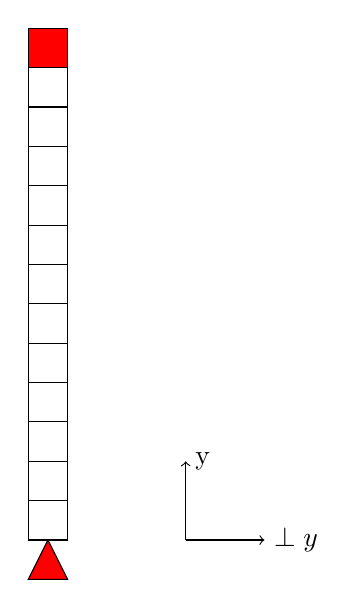
\begin{tikzpicture}
\foreach \x in {1,..., 12} \draw(0, 0.5*\x-0.5) rectangle +(.5,.5);
\filldraw[fill=red] (0, 6) rectangle +(.5,.5); 
\filldraw[fill=red] (0, -0.5) -- (0.25, 0) -- (0.5, -0.5) -- cycle;
\draw[->] (2,0) -- (2, 1) node[anchor=west] {y};
\draw[->] (2,0) -- (3, 0) node[anchor=west] {$\perp y$};
\end{tikzpicture}
\end{center}
\end{figure}

\subsection{Initial and Boundary Conditions}
\label{subsect:ic_bc}

The two problems, while having the same geometry, are different in their dominant physics.
One problem was designed to represent single-phase, single-field continuous liquid flow in a standpipe; this problem will be referred to as the "Single Phase" problem.
The second problem was designed such that high pressure liquid flashes into steam as it enters a standpipe initially filled with saturated vapor at a much lower pressure, known hereafter as the "Flashing" problem.

Table \ref{tab:ic} provides the initial conditions for the two problems.
The pressure, enthalpy, and volume-fractions for the different fields allows for a complete description of the continuity variables.
The initial velocities are set to zero.

\begin{table}[h!t]
\centering
\begin{tabular}{@{}lr@{.}lr@{.}lr@{.}lr@{.}lr@{.}l@{}} \toprule
\multirow{2}{*}{Problem} & \multicolumn{2}{c}{Pressure} & \multicolumn{2}{c}{Enthalpy}             & \multicolumn{2}{c}{$\alpha_g$} & \multicolumn{2}{c}{$\alpha_l$} & \multicolumn{2}{c}{$\alpha_e$} \\ 
                         & \multicolumn{2}{c}{[psia]} & \multicolumn{2}{c}{$[\frac{\text{Btu}}{\text{lb}_{\text{m}}}]$} & \multicolumn{2}{c}{[-]}      & \multicolumn{2}{c}{[-]}      & \multicolumn{2}{c}{[-]}      \\ \midrule
Single Phase             &  200&0                       &  355&5                                   & 0&0                            & 1&0                            & 0&0 \\
Flashing                 &  200&0                       & 1198&3                                   & 1&0                            & 0&0                            & 0&0 \\ \bottomrule  
\end{tabular}
\caption{Initial conditions for test problems.}
\label{tab:ic}
\end{table}

Each of the problems has a specified pressure-enthalpy boundary condition at the top of the stand pipe and a flow-enthalpy boundary condition at the inlet of the domain.
Table \ref{tab:bc_pe} contains the pressure, enthalpy, and composition of the pressure-enthalpy resevior. 

\begin{table}[h!t]
\centering
\begin{tabular}{@{}lr@{.}lr@{.}lr@{.}lr@{.}lr@{.}l@{}} \toprule
\multirow{2}{*}{Problem} & \multicolumn{2}{c}{Pressure} & \multicolumn{2}{c}{Enthalpy}             & \multicolumn{2}{c}{$\alpha_g$} & \multicolumn{2}{c}{$\alpha_l$} & \multicolumn{2}{c}{$\alpha_e$} \\ 
                         & \multicolumn{2}{c}{[psia]} & \multicolumn{2}{c}{$[\frac{\text{Btu}}{\text{lb}_{\text{m}}}]$} & \multicolumn{2}{c}{[-]}      & \multicolumn{2}{c}{[-]}      & \multicolumn{2}{c}{[-]}      \\ \midrule
Single Phase             &  200&0                       &  355&5                                   & 0&0                            & 1&0                            & 0&0 \\
Flashing                 &  200&0                       & 1198&3                                   & 1&0                            & 0&0                            & 0&0 \\ \bottomrule  
\end{tabular}
\caption{Pressure-enthalpy boundary conditions for test problems.}
\label{tab:bc_pe}
\end{table}

The flow-enthalpy boundary condition describes the thermodynamic state of the inflowing fluid and the rate at its flowrate.
Table \ref{tab:bc_fe} describes the inlet boundary condition for the two problems.

\begin{table}[h!t]
\centering
\begin{tabular}{@{}lr@{.}lr@{.}lr@{.}lr@{.}lr@{.}l@{}} \toprule
\multirow{2}{*}{Problem} & \multicolumn{2}{c}{Pressure} & \multicolumn{2}{c}{Enthalpy}             & \multicolumn{2}{c}{$\alpha_g$} & \multicolumn{2}{c}{$\alpha_l$} & \multicolumn{2}{c}{$\alpha_e$} \\ 
                         & \multicolumn{2}{c}{[psia]} & \multicolumn{2}{c}{$[\frac{\text{Btu}}{\text{lb}_{\text{m}}}]$} & \multicolumn{2}{c}{[-]}      & \multicolumn{2}{c}{[-]}      & \multicolumn{2}{c}{[-]}      \\ \midrule
Single Phase             &  200&0                       &  355&5                                   & 0&0                            & 1&0                            & 0&0 \\
Flashing                 & 1000&0                       &  542&6                                   & 1&0                            & 0&0                            & 0&0 \\ \bottomrule  
\end{tabular}
\caption{Flow-enthalpy boundary conditions for test problems.}
\label{tab:bc_fe}
\end{table}

The specified mass flow, $\dot{m}(t)$, at the bottom of the channels is the same for both problems. 
The is a time-dependent function give by \eqref{eqn:bc_time_func_single}.

\begin{equation}
\label{eqn:bc_time_func_single}
\dot{m}(t) = \left\{
\begin{array}{cclrcll}
 0.0           & [\frac{\text{lb}_{\text{m}}}{\text{s}}] & , &         & t & \leq 1 &[\text{s}] \\
 0.5 ( t - 1)  & [\frac{\text{lb}_{\text{m}}}{\text{s}}] & , & 1 [\text{s}] < & t & \leq 2 &[\text{s}] \\
 0.5           & [\frac{\text{lb}_{\text{m}}}{\text{s}}] & , &         & t & > 2    &[\text{s}]
\end{array}\right.
\end{equation}

Both problems adjust their initial pressure distribution to account for hydrostatic head, which is not specified on the inlet cards.
The COBRA-IE input deck for both problems can be found in \app{app:input_decks}.

\subsection{Procedure}
\label{subsect:experiments_procedure}
To determine the effect of nonlinear convergence upon the time-step size sensitivity of the solution, each problem was run for at increasingly small maximum $\Delta t$.
The material CFL limit of semi-implicit method acted as a limiter on the time-step size selected.
If the acceptable time-step size was below

\subsection{Results}
\label{subsect:results}


\section{Review}
\label{sect:review}

   % Chapter: Proof of worthiness. 
\chapter{Work Proposal}
\label{chap:proposal}
To evaluate the proposed methodology, several objectives will be pursued.
The coding of the physics based scaling for the nonlinear residual will be examined and modified as necessary to address the convergence issues such as false non-convergence.
An appropriate scaling of the Newton updates for convergence testing both within the linesearch algorithm and in the Newton loop will be determined.
The domain decomposition algorithm will be mathematically developed, coded, and evaluated.
Once the preceding three objectives have been met, a test problem will be developed to test the nonlinear refinement code as applied to a predetermined subdomain.
After the algorithmic framework has been evaluated, several geometrically complex problems with high local-nonlinearities will be developed to obtain temporal-convergence benchmarks of the legacy methodology.
The same problems will then be evaluated using the proposed algorithm to determine the efficacy of temporal-convergence criteria.
Upon completion of the temporal-convergence tests, run time tests will be conducted to determine any performance gains or losses as a result of the proposed methodology.
Parametric studies will then be conducted to determine the impact of nonlinear convergence tolerances, geometric residual imbalances, and residual thresholds for activation of nonlinear refinements.

\section{Scaling Evaluation}
\label{sect:proposal_scaling}


\section{Domain Decomposition}
\label{sect:domain_coupling}
The first step will be to implement a variation of the semi-implicit domain coupling algorithm presented in \sect{sect:code_coupling}.
The details of the derivation will need to be reworked to account for the different flow variables.

Upon completion of the implementation, a rigorous testing of the coupling methodology will be conducted.
This testing will be similar to that conducted by \citet{Weaver2002}.

\subsection{Testing}
\label{subsect:domain_testing}
To evaluate the domain decomposition capabilitites, a geometric test problem will need to be developed.
This problem should have a singular characteristic: multiple geometric components.
The problem will be a single phase run
The test problem will be run in legacy mode to obtain a standard solution.


\section{Selective Nonlinear Refinement}
\label{sect:selective_nonlinear_refinement}


\section{Evaluation}
\label{sect:future_eval}


\section{Time Line}
\label{sect:time_line}



      % Chapter: Proposal of research.

%=======================================================================
% Bibliography
%=======================================================================
\bibliographystyle{plainnat}
\bibliography{../references/references}

%=======================================================================
% Appendices
%=======================================================================
\noappendixtables
\noappendixfigures
\begin{appendices}
\chapter{COBRA-IE Input Decks}
\label{app:input_decks}

The following is the \cobra{} input file for the single-phase problem.
\singlespace
{\small \verbatiminput{files/single.inp}}

\pagebreak
The following is the \cobra{} input file for the flashing problem.
{\small \verbatiminput{files/flashing.inp}}         % Appendix: Input Decks
%\chapter{Semilog Plots}
\label{app:semilog}

\begin{figure}[h!t]
\centering
\subfloat[Nonlinear solver.]{\includegraphics[width=0.49\textwidth]{images/nl_semilogy_res.eps}
\label{fig:nl_flashing_semilog}}
\subfloat[Legacy solver.]{\includegraphics[width=0.49\textwidth]{images/cobra_semilogy_res.eps}
\label{fig:cobra_flashing_semilog}}
\caption[Semi-log plot of nonlinear residuals for the flashing problem.]{Semi-log plot of nonlinear residuals for the flashing problem.}
\label{fig:flashing_semilog_plots}
\end{figure}

\begin{figure}[h!t]
\centering
\subfloat[Nonlinear solver.]{\includegraphics[width=0.49\textwidth]{images/nl_single_semilogy_res.eps}
\label{fig:nl_single_semilog}}
\subfloat[Legacy solver.]{\includegraphics[width=0.49\textwidth]{images/cobra_single_semilogy_res.eps}
\label{fig:cobra_single_semilog}}
\caption[Semi-log plot of nonlinear residuals for the single-phase problem.]{Semi-log plot of nonlinear residuals for the single-phase problem.}
\label{fig:single_semilog_plots}
\end{figure}
%\chapter{Discrete Conservation Equations}
\label{app:residuals}

\section{Continuity Equations}

\subsection{Mass}

\begin{IEEEeqnarray}{lCr}
 \frac{\partial}{\partial t} \alpha_g \rho_g + \nabla\cdot\left(\alpha_g\rho_g\vec{U}_g\right) & = & \Gamma''' \\
 \frac{\partial}{\partial t} \alpha_l \rho_l + \nabla\cdot\left(\alpha_l\rho_l\vec{U}_l\right) & = & -(1-\eta) \Gamma''' - S''' \\
 \frac{\partial}{\partial t} \alpha_e \rho_l + \nabla\cdot\left(\alpha_e\rho_l\vec{U}_e\right) & = & -\eta \Gamma''' + S'''\\
 \frac{\partial}{\partial t} \alpha_g \rho_{nc} + \nabla\cdot\left(\alpha_g\rho_{nc}\vec{U}_g\right) & = & \Gamma''' 
 \end{IEEEeqnarray}

\begin{IEEEeqnarray}{lCl}
 % Here is the vapor mass equation.
 (\alpha \rho_v)^{n+1} + \frac{\Delta t}{V_c}\left[\sum_{J} \left[\frac{(\alpha \rho_{v})^{*}}{<\alpha \rho_v>}\right]^{n} \dot{\vec{M}}^{n+1}_{v}\cdot \vec{\hat{n}} + \sum_{K} \left[\frac{(\alpha \rho_{v})^{*}}{<\alpha \rho_v>}\right]^{n} \dot{\vec{W}}^{n+1}_{v}\cdot \vec{\hat{n}}\right] & & \nonumber \\
 = (\alpha \rho_v)^{n} + \frac{\Delta t}{V_c} \Gamma^{\,n+1} & & \\
 % Here is the gas mass equation.
 (\alpha \rho_g)^{n+1} + \frac{\Delta t}{V_c}\left[\sum_{J} \left[\frac{(\alpha \rho_{g})^{*}}{<\alpha \rho_g>}\right]^{n} \dot{\vec{M}}^{n+1}_{v}\cdot \vec{\hat{n}} + \sum_{K} \left[\frac{(\alpha \rho_{g})^{*}}{<\alpha \rho_g>}\right]^{n} \dot{\vec{W}}^{n+1}_{v}\cdot \vec{\hat{n}}\right] & & \nonumber \\
 = (\alpha \rho_g)^{n} & &  \\
 % Here is the continuous liquid mass equation.
 (\alpha_l \rho_l)^{n+1} + \frac{\Delta t}{V_c}\left[\sum_{J} \left[\frac{(\alpha_l \rho_{l})^{*}}{<\alpha_l \rho_l>}\right]^{n} \dot{\vec{M}}^{n+1}_{l}\cdot \vec{\hat{n}} + \sum_{K} \left[\frac{(\alpha_l \rho_{l})^{*}}{<\alpha_l \rho_l>}\right]^{n} \dot{\vec{W}}^{n+1}_{l}\cdot \vec{\hat{n}}\right] & & \nonumber \\
 = (\alpha_l \rho_l)^{n} + \frac{\Delta t}{V_c} \left(S_{D}^{n+1} - (1-\eta^{n})\Gamma^{\,n+1}_{l} - S_{E}^{n+1}\right) & & \\
 % Here is the entrained liquid mass equation.
 (\alpha_e \rho_l)^{n+1} + \frac{\Delta t}{V_c}\left[\sum_{J} \left[\frac{(\alpha_e \rho_{l})^{*}}{<\alpha_e \rho_l>}\right]^{n} \dot{\vec{M}}^{n+1}_{e}\cdot \vec{\hat{n}} + \sum_{K} \left[\frac{(\alpha_e \rho_{l})^{*}}{<\alpha_e \rho_l>}\right]^{n} \dot{\vec{W}}^{n+1}_{e}\cdot \vec{\hat{n}}\right] & & \nonumber \\
 = (\alpha_e \rho_l)^{n} + \frac{\Delta t}{V_c} \left(S_{E}^{n+1} - \eta^{n}\Gamma^{\,n+1}_{e} - S_{D}^{n+1}\right)& & 
 \end{IEEEeqnarray}

\subsection{Energy}

\begin{IEEEeqnarray}{Cr}
 \frac{\partial}{\partial t}\left(\alpha_g (\rho_v h_v+\rho_{nc} h_{nc})\right)+\nabla\cdot\left(\alpha_g(\rho_v h_v + \rho_{nc} h_{nc}) \vec{U}_g\right) & \nonumber \\
 = \Gamma'''h'_{v} + q'''_{i,v} + q'''_{gl} + q'''_{wg} + \alpha_g \frac{\partial P}{\partial t} & \\
 \frac{\partial}{\partial t}\left((\alpha_e +\alpha_l) \rho_l h_l\right)+\nabla\cdot\left(\alpha_l\rho_l h_l \vec{U}_l\right)+\nabla\cdot\left(\alpha_e\rho_l h_l \vec{U}_e\right)  \nonumber \\
 = \Gamma'''h'_{v} + q'''_{i,v} + q'''_{gl} + q'''_{wg} + \alpha_g \frac{\partial P}{\partial t} &
 \end{IEEEeqnarray}

\begin{IEEEeqnarray}{ll}
 % Here be the gas equations.
  & (\alpha_g (\rho_v h_v + \rho_{nc} h_{nc}) )^{n+1} - \alpha_{g}^{n}P^{\;n+1} \nonumber \\
 +& \frac{\Delta t}{V_c} \sum_{J} \left(\frac{(\alpha_g (\rho_v h_v + \rho_{nc} h_{nc}) )^{*}}{<\alpha_g (\rho_v h_v + \rho_{nc} h_{nc}) >}\right)^{n} \dot{\vec{M}}^{n+1}_{v}\cdot \vec{\hat{n}} \nonumber \\
 +& \frac{\Delta t}{V_c} \sum_{K} \left(\frac{(\alpha_g (\rho_v h_v + \rho_{nc} h_{nc}) )^{*}}{<\alpha_g (\rho_v h_v + \rho_{nc} h_{nc}) >}\right)^{n} \dot{\vec{W}}^{n+1}_{v}\cdot \vec{\hat{n}} \nonumber \\
 =& (\alpha_g (\rho_v h_v + \rho_{nc} h_{nc}) )^{n} - \alpha_{g}^{n}P^{\;n} + \frac{\Delta t}{V_c}\left(q^{n}_{wg} + q^{n}_{i,v} + \Gamma^{\,n}h'^{\,n}_{v} + q^{n}_{gl}\right)\\
 % Here be the liquid equations.
  & ((\alpha_e +\alpha_l) \rho_l h_l)^{n+1} - (\alpha_e +\alpha_l)^{n}P^{\;n+1} \nonumber \\
 +& \frac{\Delta t}{V_c} \sum_{J}\left[  \left(\frac{(\alpha_l \rho_l h_l )^{*}}{<\alpha_l \rho_l h_l >}\right)^{n} \dot{\vec{M}}^{n+1}_{l}\cdot \vec{\hat{n}}+ \left(\frac{(\alpha_e \rho_l h_l )^{*}}{<\alpha_e \rho_l h_l >}\right)^{n} \dot{\vec{M}}^{n+1}_{e}\cdot \vec{\hat{n}}\right] \nonumber \\
 +& \frac{\Delta t}{V_c} \sum_{K}\left[  \left(\frac{(\alpha_l \rho_l h_l )^{*}}{<\alpha_l \rho_l h_l >}\right)^{n} \dot{\vec{W}}^{n+1}_{l}\cdot \vec{\hat{n}}+ \left(\frac{(\alpha_e \rho_l h_l )^{*}}{<\alpha_e \rho_l h_l >}\right)^{n} \dot{\vec{W}}^{n+1}_{e}\cdot \vec{\hat{n}}\right] \nonumber \\
 =& ((\alpha_e +\alpha_l) \rho_l h_l)^{n} - (\alpha_e +\alpha_l)^{n}P^{\;n} + \frac{\Delta t}{V_c}\left(q^{n}_{wl} + q^{n}_{i,l} -\Gamma^{\,n}h'^{\,n}_{l} - q^{n}_{gl}\right)
 \end{IEEEeqnarray}

 \begin{IEEEeqnarray}{lr}
 \frac{\partial }{\partial t} \left(\alpha_g (\rho_v + \rho_{nc}) \Vec{U}_g \right) + \nabla\cdot\left(\alpha_g (\rho_v + \rho_{nc}) \vec{U}_g \vec{U}_g \right) = &\nonumber \\
 -\alpha_g\;\nabla P + \alpha_g (\rho_v + \rho_{nc}) \vec{g} - \tau^{'}_{wg}-\tau^{'}_{I_{gl}} - \tau^{'}_{I_{ge}} + \Gamma''' \vec{U}^{'} & \\
 \frac{\partial }{\partial t} \left(\alpha_l \rho_l \Vec{U}_l \right) + \nabla\cdot\left(\alpha_l \rho_l \vec{U}_l \vec{U}_l \right) = &\nonumber \\
 -\alpha_l\;\nabla P + \alpha_l \rho_l \vec{g} - \tau^{'}_{wl} + \tau^{'}_{I_{gl}} -\left((1-\eta)\Gamma'''\vec{U}'\right) - S'''\vec{U}'& \\
 \frac{\partial }{\partial t} \left(\alpha_e \rho_l \Vec{U}_e \right) + \nabla\cdot\left(\alpha_e \rho_l \vec{U}_e \vec{U}_e \right) = &\nonumber \\
 -\alpha_e\;\nabla P + \alpha_e \rho_l \vec{g} - \tau^{'}_{wl} + \tau^{'}_{I_{ge}} -\left(\eta\Gamma'''\vec{U}'\right) + S'''\vec{U}'&
 \end{IEEEeqnarray}

 \begin{IEEEeqnarray}{rCl}
 F_g(\Vec{x}^{n+1}) & = & \overbrace{E_g({\Vec{x}^{n}})}^{\text{Purely explicit terms}}-\overbrace{A_{mom,j}\Delta z_j\left[ \alpha_g^n\frac{P_{J+1}^{n+1}-P_{J}^{n+1}}{\Delta z_j}\right]}^{\text{Semi-Implicit Pressure Term}}  \\
 & - & \overbrace{A_{mom,j}\Delta z_j\left[ \frac{dP}{dz}\bigg|_{w,g}^{*}+\frac{dP}{dz}\bigg|_{i,lg}^{*}+\frac{dP}{dz}\bigg|_{i,eg}^{*}\right]}^{\text{Semi-Implicit Drag Terms}}\nonumber \\
 & + & \overbrace{\mathcal{S}p^{n+1}_{g,j}}^{\text{Implicit Source Term}} -\overbrace{\frac{\left(M_{g,j}^{n+1}-M_{g,j}^{n}\right)}{\Delta t}\Delta z}^{\text{Time rate of change}}\nonumber \\
 & = &  0 \nonumber
 \end{IEEEeqnarray}  % Appendix: Nonlinear Math
%\chapter{Two-phase Flow Equations}
\label{app:two_phase_flow}

Two phase flow is crazy.

\section{blarger}
\label{sect:blarger}
The details of two phase flow are given here.

      % Appendix: Two Phase Flow
%\chapter{Newton Steps}
\label{app:newton}

 Linearization of the axial momentum equations in COBRA-IE.

\begin{IEEEeqnarray}{rCl}
  \vec{x}_k & = \begin{bmatrix}
   \dot{\vec{M}}_k \\
   \Delta \text{P}_k
 \end{bmatrix}\ & = \begin{bmatrix}
 \dot{M}_{l,k}\\
 \dot{M}_{g,k}\\
 \dot{M}_{e,k}\\
 \Delta \text{P}_{k}
 \end{bmatrix}
 \end{IEEEeqnarray}

 Note: 

 \begin{IEEEeqnarray}{rCCCr}
 \vec{L}(\vec{x}_{k}) & = & \mat{L}\;\dot{\vec{M}}_{k} + \vec{b}\Delta\text{P}_{k} \nonumber \\
 \frac{\partial}{\partial \Delta\text{P}_{k}}\left[\vec{b} \Delta \text{P}_{k}\right] & = & \vec{b} \nonumber \\
 \frac{\partial\; \vec{N}(\vec{x}_{k})}{\partial \vec{x}_{k}} & = & \frac{\partial\; \vec{N}(\vec{x}_{k})}{\partial \dot{\vec{M}}_{k}} & = & \mat{N}(\dot{\vec{M}}_{k}) \nonumber \\
 \mat{J}^{*}_{k} & = & \frac{\partial\; \vec{F}(\vec{x}_{k})}{\partial \dot{\vec{M}_{k}}} & = & \mat{L} + \mat{N}(\dot{\vec{M}}_{k})  \nonumber \\
 \mat{J}_{\,k}\delta \vec{x} & = & \frac{\partial\; \vec{F}(\vec{x}_{k})}{\partial \vec{x}_{k}}\delta\vec{x} & = & \mat{J}^{*}_{\,k}\delta(\dot{\vec{M}}) + \vec{b}\delta(\Delta \text{P})\nonumber
 \end{IEEEeqnarray}



Current View Point

\begin{IEEEeqnarray}{rCl}
 0 & = & \vec{F}(\vec{x}_{k+1}) \nonumber \\
 0 & = & \vec{F}(\vec{x}_{k+1}) =  \vec{E} + \vec{L}(\vec{x}_{k+1}) + \vec{N}(\vec{x}_{k+1})  \nonumber \\
 0 & = & \vec{E} + \vec{L}(\vec{x}_{k+1}) + \vec{N}(\vec{x}_{k+1}) \nonumber \\
 0 & = & \vec{E} + \mat{L}\;\dot{\vec{M}}_{k+1} + \vec{b}\Delta\text{P}_{k+1} + \vec{N}(\vec{x}_{k+1}) \nonumber \\
 0 & = & \vec{E} + \mat{L}\;\dot{\vec{M}}_{k+1} + \vec{b}\Delta \text{P}_{k} + \frac{\partial\left[ \vec{b}\Delta\text{P}_{k+1}\right]}{\partial\,\Delta \text{P}_{k+1}}\delta(\Delta \text{P}) + \vec{N}(\vec{x}_{k}) + \frac{\partial \left[ \vec{N}(\vec{x}_{k+1})\right]}{\partial\, \vec{x}_{k+1}}\left[\vec{x}_{k+1}-\vec{x}_{k}\right] \nonumber
 \end{IEEEeqnarray}

 \begin{IEEEeqnarray}{rCl}
  \mat{L}\;\dot{\vec{M}}_{k+1} + \mat{N}(\dot{\vec{M}}_{k})\;\dot{\vec{M}}_{k+1} & = & -\vec{E} - \vec{b}\Delta \text{P}_{k} - \vec{N}(\vec{x}_{k}) - \vec{b}\delta(\Delta \text{P}) + \mat{N}(\dot{\vec{M}}_{k})\dot{\vec{M}}_{k} \nonumber \\
  \left[\mat{L} + \mat{N}(\dot{\vec{M}}_{k})\right]\dot{\vec{M}}_{k+1} & = & - \left[\vec{E} + \vec{b}\Delta \text{P}_{k} + \vec{N}(\vec{x}_{k}) - \mat{N}(\dot{\vec{M}}_{k})\;\dot{\vec{M}}_{k}\right] - \vec{b}\delta(\Delta \text{P}) \nonumber \\
  \mat{J}^{*}_{\,k}\; \dot{\vec{M}}_{k+1} & = &  -\vec{f} - \vec{b}\delta(\Delta \text{P}) \nonumber \\
 \dot{\vec{M}}_{k+1} & = &  \underbrace{-\mat{J}_{\,k}^{-*}\;\vec{f}}_{\dot{\vec{M}}^{\widetilde{n+1}}_{\,k}} \underbrace{- \mat{J}^{-*}_{\,k}\;\vec{b}}_{\frac{d \dot{\vec{M}}_{k}}{d \Delta \text{P}}}\delta(\Delta \text{P}) \nonumber \\
 \dot{\vec{M}}_{k+1} & = &  \dot{\vec{M}}^{\widetilde{n+1}}_{\,k} + \frac{d \dot{\vec{M}}_{k}}{d \Delta \text{P}}\delta(\Delta \text{P}) \nonumber 
 \end{IEEEeqnarray}

Relation between Newton step and current formulation.

 \begin{IEEEeqnarray}{rCl}
 \left[\mat{L} + \mat{N}(\dot{\vec{M}}_{k})\right]\dot{\vec{M}}_{k+1} & = & - \left[\vec{E} + \mat{L}\;\dot{\vec{M}}_{k} + \vec{b}\Delta \text{P}_{k} + \vec{N}(\vec{x}_{k}) \right] \nonumber \\
 & & - \vec{b}\delta(\Delta \text{P}) + \mat{L}\;\dot{\vec{M}}_{k} + \mat{N}(\dot{\vec{M}}_{k})\;\dot{\vec{M}}_{k} \nonumber \\
 \left[\mat{L} + \mat{N}(\dot{\vec{M}}_{k})\right]\dot{\vec{M}}_{k+1} & = & - \vec{F}(\vec{x}_{k}) - \vec{b}\delta(\Delta \text{P}) + \left[\mat{L} + \mat{N}(\dot{\vec{M}}_{k})\right]\;\dot{\vec{M}}_{k} \nonumber \\
 \mat{J}^{*}_{\,k}\,\dot{\vec{M}}_{k+1} & = & - \vec{F}(\vec{x}_{k}) - \vec{b}\delta(\Delta \text{P}) + \mat{J}^{*}_{\,k}\;\dot{\vec{M}}_{k} \nonumber \\
 \dot{\vec{M}}_{k+1} & = & \underbrace{\dot{\vec{M}}_{k} - \mat{J}_{\,k}^{-*} \vec{F}(\vec{x}_{k})}_{\dot{\vec{M}}^{\widetilde{n+1}}_{\,k}} \underbrace{- \mat{J}_{\,k}^{-1}\vec{b}}_{\frac{d \dot{\vec{M}}_{k}}{d \Delta \text{P}}}\delta\text{P} \nonumber \\
 \dot{\vec{M}}_{k+1} & = &  \dot{\vec{M}}^{\widetilde{n+1}}_{\,k} + \frac{d \dot{\vec{M}}_{k}}{d \Delta \text{P}}\delta(\Delta \text{P}) \nonumber 
 \end{IEEEeqnarray}


Equivalence with a Newton step.

 \begin{IEEEeqnarray}{rCl}
 \left[\mat{L} + \mat{N}(\dot{\vec{M}}_{k})\right]\dot{\vec{M}}_{k+1} & = & - \left[\vec{E} + \mat{L}\;\dot{\vec{M}}_{k} + \vec{b}\Delta \text{P}_{k} + \vec{N}(\vec{x}_{k}) \right] \nonumber \\
 & & - \vec{b}\delta(\Delta \text{P}) + \mat{L}\;\dot{\vec{M}}_{k} + \mat{N}(\dot{\vec{M}}_{k})\;\dot{\vec{M}}_{k} \nonumber \\
 \left[\mat{L} + \mat{N}(\dot{\vec{M}}_{k})\right]\dot{\vec{M}}_{k+1} & = & - \vec{F}(\vec{x}_{k}) - \vec{b}\delta(\Delta \text{P}) + \left[\mat{L} + \mat{N}(\dot{\vec{M}}_{k})\right]\;\dot{\vec{M}}_{k} \nonumber \\
 \mat{J}^{*}_{\,k}\,\dot{\vec{M}}_{k+1} & = & - \vec{F}(\vec{x}_{k}) - \vec{b}\delta(\Delta \text{P}) + \mat{J}^{*}_{\,k}\;\dot{\vec{M}}_{k} \nonumber \\
 \mat{J}^{*}_{\,k}\,\left[\dot{\vec{M}}_{k+1}-\dot{\vec{M}}_{k} \right] & = & - \vec{F}(\vec{x}_{k}) - \vec{b}\delta(\Delta \text{P}) \nonumber \\
 \mat{J}^{*}_{\,k}\,\delta(\dot{\vec{M}}) + \vec{b}\delta(\Delta \text{P})  & = & - \vec{F}(\vec{x}_{k})  \nonumber \\
 \mat{J}_{\,k}\,\delta\vec{x} + \vec{b}\delta(\Delta \text{P})  & = & - \vec{F}(\vec{x}_{k})  \nonumber 
 \end{IEEEeqnarray}

 \begin{align}
 \begin{bmatrix} 
 \DerivParOne{\vec{I}_{l}}{\vec{\dot{M}}_{l}} & \DerivParOne{\vec{I}_{l}}{\vec{\dot{M}}_{g}}  & \DerivParOne{\vec{I}_{l}}{\vec{\dot{M}}_{e}} & \DerivParOne{\vec{I}_{l}}{\Delta P}\\
 \DerivParOne{\vec{I}_{g}}{\vec{\dot{M}}_{l}} & \DerivParOne{\vec{I}_{g}}{\vec{\dot{M}}_{g}}  & \DerivParOne{\vec{I}_{g}}{\vec{\dot{M}}_{e}} & \DerivParOne{\vec{I}_{g}}{\Delta P}\\
 \DerivParOne{\vec{I}_{e}}{\vec{\dot{M}}_{l}} & \DerivParOne{\vec{I}_{e}}{\vec{\dot{M}}_{g}}  & \DerivParOne{\vec{I}_{e}}{\vec{\dot{M}}_{e}} & \DerivParOne{\vec{I}_{e}}{\Delta P}
 \end{bmatrix}_{0}
 \cdot
 \begin{bmatrix}
 \Delta \vec{\dot{M}}_l \\
 \Delta \vec{\dot{M}}_g \\
 \Delta \vec{\dot{M}}_e \\
 \Delta P
 \end{bmatrix}_{k\rightarrow k+1} & =
 -\begin{bmatrix}
 \vec{E}_{l} \\
 \vec{E}_{g} \\
 \vec{E}_{e}
 \end{bmatrix} -
 \begin{bmatrix}
 \vec{I}_{l} \\
 \vec{I}_{g} \\
 \vec{I}_{e}
 \end{bmatrix}_{k} \\ 
 % HERE IS A SEPERATE EQUATION
 \begin{bmatrix} 
 \DerivParOne{\vec{I}_{l}}{\vec{\dot{M}}_{l}} & \DerivParOne{\vec{I}_{l}}{\vec{\dot{M}}_{g}}  & \DerivParOne{\vec{I}_{l}}{\vec{\dot{M}}_{e}} \\
 \DerivParOne{\vec{I}_{g}}{\vec{\dot{M}}_{l}} & \DerivParOne{\vec{I}_{g}}{\vec{\dot{M}}_{g}}  & \DerivParOne{\vec{I}_{g}}{\vec{\dot{M}}_{e}} \\
 \DerivParOne{\vec{I}_{e}}{\vec{\dot{M}}_{l}} & \DerivParOne{\vec{I}_{e}}{\vec{\dot{M}}_{g}}  & \DerivParOne{\vec{I}_{e}}{\vec{\dot{M}}_{e}}
 \end{bmatrix}_{0}
 \cdot
 \begin{bmatrix}
 \Delta \vec{\dot{M}}_l \\
 \Delta \vec{\dot{M}}_g \\
 \Delta \vec{\dot{M}}_e
 \end{bmatrix}_{k\rightarrow k+1} & =
 -\vec{E} -
 \vec{I}_{k} -
 \begin{bmatrix}
 \DerivParOne{\vec{I}_{l}}{\Delta P} \\
 \DerivParOne{\vec{I}_{g}}{\Delta P} \\
 \DerivParOne{\vec{I}_{e}}{\Delta P}
 \end{bmatrix}_{0}
 \Delta P_{k \rightarrow k+1} \\
 % HERE IS A SEPERATE EQUATION
 \mat{J}_{\,0}
 \cdot
 \begin{bmatrix}
 \Delta \vec{\dot{M}}_l \\
 \Delta \vec{\dot{M}}_g \\
 \Delta \vec{\dot{M}}_e
 \end{bmatrix}_{k\rightarrow k+1} & =
 -\vec{E} -
 \vec{I}_{k} -
 \vec{p}_{0}
 \Delta P_{k \rightarrow k+1} \\
 % HERE IS A SEPERATE EQUATION
 \begin{bmatrix}
 \Delta \vec{\dot{M}}_l \\
 \Delta \vec{\dot{M}}_g \\
 \Delta \vec{\dot{M}}_e
 \end{bmatrix}_{k\rightarrow k+1} & =
 -\mat{J}_{\,0}^{-1}\left(\vec{E} + \vec{I}_{k}\right) -
 \mat{J}_{\,0}^{-1} \cdot \vec{p}_{0} \Delta P_{k \rightarrow k+1} 
  \end{align}
  \begin{align}
 % HERE IS A SEPERATE EQUATION
 \vec{\dot{M}}^{n+1}_{k+1}- \vec{\dot{M}}^{n+1}_{k} & =
 -\mat{J}_{\,0}^{-1}\left(\vec{E} + \vec{I}_{k}\right) -
 \mat{J}_{\,0}^{-1} \cdot \vec{p}_{0} \Delta P_{k \rightarrow k+1}\\
 % HERE IS A SEPERATE EQUATION
 \vec{\dot{M}}^{n+1}_{k+1} & =
 \underbrace{\vec{\dot{M}}^{n+1}_{k} -\mat{J}_{\,0}^{-1}\left(\vec{E} + \vec{I}_{k}\right)}_{\vec{\dot{M}}^{*}_{k}} - \underbrace{\mat{J}_{\,0}^{-1} \cdot \vec{p}_{0}}_{\frac{\partial \vec{\dot{M}}}{\partial \Delta P}} \Delta P_{k \rightarrow k+1} \\
 % HERE IS A SEPERATE EQUATION
 \vec{\dot{M}}^{n+1}_{k+1} & =
 \underbrace{-\mat{J}_{\,0}^{-1}\cdot \vec{E} + \vec{\dot{M}}^{n+1}_{k} - \mat{J}^{-1}_{\,0}\cdot \vec{I}_{k}}_{\vec{\dot{M}}^{n+1}_{*}} - \underbrace{\mat{J}_{\,0}^{-1} \cdot \vec{p}_{0}}_{\frac{\partial \vec{\dot{M}}}{\partial \Delta P}} \Delta P_{k \rightarrow k+1}
 \end{align}

 \begin{align}
 % HERE IS A SEPERATE EQUATION
 \vec{\dot{m}}^{n+1}_{k+1} & =
 \underbrace{-\mat{J}_{\,0}^{-1}\cdot \vec{E} + \vec{\dot{m}}^{n+1}_{k} - \mat{J}_{\,0}\cdot \vec{I}_{k}}_{\vec{\dot{m}}^{n+1}_{*}} - \underbrace{\mat{J}_{\,0}^{-1} \cdot \vec{p}_{0}}_{\frac{\partial \vec{\dot{m}}}{\partial \Delta P}} \Delta P_{k \rightarrow k+1} \\
 % HERE IS A SEPERATE EQUATION
 \vec{\dot{m}}^{n+1}_{k+1} & =
 \underbrace{-\mat{J}_{\,0}^{-1}\cdot \vec{E} + \vec{\dot{m}}^{n+1}_{k} - \mat{J}_{\,0}\cdot \vec{I}_{k}}_{\vec{\dot{m}}^{n+1}_{*}} - \frac{\partial \vec{\dot{m}}}{\partial \Delta P}\bigg|_{0} \Delta P_{k \rightarrow k+1} \\
 % HERE IS A SEPERATE EQUATION
 \vec{\dot{m}}^{n+1}_{k+1} & =
 \underbrace{-\mat{J}_{\,0}^{-1}\cdot \vec{E} + \left(\mat{I} - \mat{J}^{-1}_{\,0}\cdot \mat{\alpha}_{0}\right)\cdot\vec{x}^{n+1}_{k}}_{\vec{\dot{m}}^{n+1}_{*}} - \frac{\partial \vec{\dot{m}}}{\partial \Delta P}\bigg|_{0} \Delta P_{k \rightarrow k+1}
\end{align}


 \begin{align}
 \Mat{J}_{0} & \equiv -\frac{2 A_{mom}\Delta t}{\Delta z}\cdot \nonumber \\
 &\cdot \begin{bmatrix} 
 K^{n}_{w,l} + \frac{K^{n}_{i,lg}}{\Ave{\alpha\rho}^{n}_{l}} +\frac{1}{2} &  -\frac{K^{n}_{i,lg}}{\Ave{\alpha\rho}^{n}_{g}} & 0\\
 -\frac{K^{n}_{i,lg}}{\Ave{\alpha\rho}^{n}_{l}} &  K^{n}_{w,g} + \frac{K^{n}_{i,lg}}{\Ave{\alpha\rho}^{n}_{g}}+\frac{K^{n}_{i,eg}}{\Ave{\alpha\rho}^{n}_{g}} +\frac{1}{2} & -\frac{K^{n}_{i,eg}}{\Ave{\alpha\rho}^{n}_{e}}\\
 0 & -\frac{K^{n}_{i,eg}}{\Ave{\alpha\rho}^{n}_{g}} &  K^{k}_{w,e} + \frac{K^{n}_{i,eg}}{\Ave{\alpha\rho}^{n}_{e}}+\frac{1}{2}\\
 \end{bmatrix}
 \end{align}              % Appendix: Newton Formulation
\end{appendices}

%=======================================================================
% End Document
%=======================================================================
\end{document}
